Strojové učení (anglicky Machine Learning, \gls{ML}) představuje odvětví umělé
inteligence, které se zaměřuje na vytváření matematických modelů a zvyšování
jejich přesnosti predikce na základě předchozích zkušeností. Tyto zkušenosti se
získávají retrospektivně z dostupných dat (trénovacích dat), která se využívají
k formulaci pravidel a identifikaci charakteristických rysů nebo vztahů v
datech. Proces učení zahrnuje techniky, které vyplývají z  oborů informatiky,
statistiky, pravděpodobnosti nebo optimalizace. Využití algoritmů strojového
učení se neustále rozšiřuje v mnoha oblastech díky rostoucí dostupnosti online
dat a snižování nákladů na výpočetní zdroje. Rozsah oblastí použití zahrnuje
široké spektrum oborů, včetně zdravotnictví.

Tato kapitola slouží jako úvod do vybraných základních pojmů strojového učení s
cílem vytvořit teoretický náhled pro podporu pochopení problematiky v
korespondujících částech práce. Detailněji byly principy a náležitosti
strojového učení již popsány v
literatuře~\cite{Aurelien2022,Murphy2012,Goodfellow2016}.

\subsection{Typy systémů strojového učení}
Různorodost scénářů strojového učení je charakterizována rozdíly v povaze
trénovacích dat, způsobu trénování a kritériích hodnocení. Každý přístup je
vhodný pro řešení určité kategorie problémů a představuje své vlastní
charakteristické výhody a omezení. V následujících podkapitolách jsou rozebrány
primárně dvě nejrozšířenější formy přístupů k učení, tj. učení s učitelem
(anglicky Supervised Learning) a učení bez učitele (anglicky Unsupervised
Learning).

\subsubsection{Učení s učitelem}
\label{subsubsec:supervised_learning}
Učení s učitelem je typ strojového učení, během kterého se využívají právě
taková trénovací data, která mají anotovanou výstupní proměnnou. Úkolem je zde
aproximovat mapovací funkci $h$, která predikuje výstupní proměnnou na základě
vstupní proměnné $X$. K aproximaci mapovací funkce jsou použita označená
trénovací data, která se skládají z $n$ párů vstupních a výstupních proměnných.
Cílem je získat přesné predikce jak pro trénovací, tak pro úplně nová data.
Formálně lze tedy tvrdit, že hledáme funkci:
\begin{equation}
    h:\mathbb{R}^d \rightarrow \mathcal{C}
\end{equation}
tak, že pro každou novou dvojici vstupu a výstupu $(x,y)$ vybranou z
$\mathcal{P}$ platí $h(X) ≈ y$, kde $\mathbb{R}^d$ je je $d$-rozměrný příznakový
prostor a $\mathcal{C}$ je prostor všech možných anotací. Zároveň předpokládáme,
že tyto dvojice pocházejí z neznámého rozdělení
$\mathcal{P}$~\cite{Murphy2012}.

\subsubsection{Učení bez učitele}
Cílem učení bez učitele je najít vzory v neanotovaných datech bez definovaného
výstupu. Výsledkem tohoto typu učení mohou být struktury nebo vztahy v datech.
Vyhodnocování výkonu natrénovaného modelu je v tomto případě, bez označených
dat, často náročné. Běžnou úlohou pro tento typ učení je shlukování, které
seskupuje podobné data do shluků. Shlukování se používá například pro segmentaci
obrazových dat a provádí se pomocí algoritmů, jako je hustotní prostorové
shlukování (\gls{DBSCAN}), k-means nebo hierarchické shlukování.

\begin{figure}[!htb]
    \begin{center}
        \begin{tikzpicture}[board/.style={minimum width=6em,minimum height=1em,
                        draw,fill=gray!20,path picture={
                                \foreach \XX in {0,...,5}
                                    {\ifnum\XX>0
                                            \draw ([xshift=\XX*1em]path picture bounding box.north west)
                                            -- ([xshift=\XX*1em]path picture bounding box.south west);
                                        \fi
                                        \ifnum\XX=#1
                                            \draw[fill=blue!50] ([xshift=\XX*1em]path picture bounding box.north west)
                                            rectangle ([xshift=\XX*1em-1em]path picture bounding box.south west);
                                        \fi}
                            },pin={[name=pin-#1]right:Vyhodnocení$_{#1}$},scale=1.2},
                box/.style={draw,minimum size=1.2em,fill=blue!50,label={[node
                                        font=\tiny,align=center]#1}},
                2box/.style={rectangle split, rectangle split parts=2, draw,minimum
                        width=#1}, 2ell/.style={ellipse split,draw},
                every pin edge/.style={-stealth},font=\sffamily]
            \matrix[matrix of nodes,nodes in empty cells,nodes={anchor=center},
            row sep=1ex,column sep=1em,inner xsep=0.3em] (m) {
            1. & |[board=1]| \\
            2. & |[board=2]| \\
            3. & |[board=3]| \\
            4. & |[board=4]| \\
            5. & |[board=5]| \\
            };
            \draw[semithick,decorate,decoration={brace,mirror,raise=1pt}] (m-1-2.north east)
            -- ++ (-4.8em,0)
            node[midway,above=1ex,align=center] (TF) {Trénovací\\ vzorek};
            \node[left=1em of TF,align=center] (VF) {Validační\\ vzorek};
            \node[anchor=south,rotate=90] at (m.west){$k$-iterace};
            \draw (VF) -- ([xshift=0.6em]m-1-2.north west);
            \draw[semithick,decorate,decoration={brace,mirror,raise=1pt}] (m-5-2.south west) -- ++ (4.8em,0)
            coordinate[midway,below=1ex](5f);
            \draw[semithick,decorate,decoration={brace,raise=1pt}] (m.north east)
            -- (m.south east)  node[midway,right=1ex,2box=4em,draw=none,anchor=text west,
                rectangle split part align={left}]{Vyhodnocení
                \nodepart{two}$=\sum\limits_{i=1}^5\textsf{Vyhodnocení}_i$};
            \node[below=2em of m-5-2.south west,2box,fill=gray!20] (2box) {Trénovací vzorek\nodepart{two}Značky trénovacího vzorku};
            \node[below=2em of 2box,2ell,inner ysep=-0.2ex] (2ell){
                \begin{tabular}{@{}c@{}}
                    Hodnoty \\ hyperparametrů
                \end{tabular}
                \nodepart{lower}
                \begin{tabular}{@{}c@{}}
                    \textbf{Vybraný algortimus} \\
                    \textbf{strojového učení}
                \end{tabular}};
            \node[below=2em of 2ell,regular polygon,regular polygon
                sides=6,fill,text=white] (6gon) {Model};
            \draw[>=stealth]  (5f) edge[->] (2box) (2box) edge[->] (2ell) (2ell) edge[->] (6gon);
            %
            \draw[semithick,decorate,decoration={brace,mirror,raise=1pt}]
            (pin-5.south west) -- (pin-5.south east) coordinate[midway,below=1.2ex] (pf)
            node[midway,below=2em,box=left:{Validační\\ vzorek}](b1){};
            \node[right=4em of b1,box=above:Predikce,yshift=-0.5ex] (b2){};
            \node[below=4em of b2,box=below:{Validační\\ značky}] (b3){};
            \path (b2) -- (b3) coordinate[midway,right=1em] (aux)
            node[right=1em of aux] (PF) {Vyhodnocení};
            \draw[-stealth] (b2.east) -| (aux) |- (b3.east) (aux) -- (PF);
            \node[below=0.5em of b1,regular polygon,regular polygon sides=6,fill,text=white] (6gon2) {Model};
            \path coordinate[left=1em of b2] (aux2);
            \draw[-stealth] (6gon2.east) -| (aux2) |- (b1.east) (aux2) -- (b2);
            \draw[-stealth] (pf) -- (b1);
        \end{tikzpicture}
        \caption{Obecné schéma procesu trénování modelu a optimalizací
            hyperparametrů s využitím k-násobné křížové
            validace~\cite{crossvalidation}}
        \label{fig:cross-validation}
    \end{center}
\end{figure}


\subsection{Trénování a testování modelů}
Vyhodnocování modelů strojového učení je pro jejich úspěšnost klíčové. Aby bylo
zajištěno, že model dokáže efektivně predikovat i nová data, nikoli pouze data
využita během jeho trénování, provádí se tzv. \emph{train-test} rozdělení. To
zahrnuje ponechání části dat jako testovací množiny, kterou model během
trénování nepoužil, a její následné použití k vyhodnocení schopnosti modelu
generalizace porovnáním jeho predikce se skutečnými hodnotami.

Běžně se využívá rozdělení trénovací a testovací množiny v poměru 80:20 z
náhodně vybraných dat. Dále se někdy využívá validační množina (15-20 \%
trénovací množiny) pro účely ladění hyperparametrů. Nejúspěšnější model se na
základě validační množiny natrénuje pomocí nalezených hyperparametrů. Nakonec se
model vyhodnotí na dosud nevyužité testovací množině. Hyperparametry a jejich
optimalizace jsou rozebrány v samostatné
podkapitole~\ref{subsec:hyperparametry}.

\subsubsection{Křížová validace} %  Cross-validation
Přístup rozdělení dat z předchozí sekce je efektivní, ale opomíjí jeden problém:
existuje mnoho možných kombinací trénovací a testovací sady a tato metoda zkoumá
pouze jednu. Data mohla být tedy náhodně rozdělena nereprezentativním způsobem.
Odpovědí na tento problém je křížová validace (anglicky cross-validation,
\gls{CV}), která eliminuje závislost na rozdělení dat. Cílem křížové validace je
vyhodnotit a porovnat výkon různých modelů na stejném datovém souboru a najít
tak optimální nastavení hyperparametrů pro daný model.

Křížová validace se skládá ze tří hlavních kroků: rozdělení datového souboru na
$k$ částí, trénování modelu na $k - 1$ částech dat a vyhodnocování výkonu modelu
na zbývající (validace) části dat. Tyto kroky se opakují $n$ krát, přičemž každá
část dat se použije jednou jako validace. Výsledkem křížové validace je průměrný
výkon modelu na všech $k$ částech validace. Existuje celá řada způsobů provedení
křížové validace: K-Fold, Leave One Out (LOO), Stratified Shuffle Split, Leave P
Groups Out, a další, které byly jíž popsány v~\cite{Aurelien2022}.

Křížová validace má řadu výhod oproti jiným metodám optimalizace hyperparametrů,
jako je například mřížkové nebo náhodné vyhledávání popsané v dalších
kapitolách. Mezi tyto výhody patří:
\begin{itemize}
    \item Objektivní hodnocení výkonu modelu na stejných datech~\cite{tibshirani1993}.
    \item Minimalizace rizika přeučení~\cite{anguita2013}.
    \item Efektivní využití všech dat k hodnocení výkonu modelu~\cite{kohavi1995}.
\end{itemize}

V praxi se křížová validace často používá pro optimalizaci hyperparametrů nejen
jednoho, ale i více modelů současně a následně porovnání jejich výkonu.

\subsubsection{Přeučení a nedoučení}
\label{subsubsec:underoverfitting}
Přeučení (anglicky overfitting) a nedoučení (anglicky underfitting) jsou dva
hlavní problémy, které se mohou vyskytnout při trénování modelů strojového
učení. Tyto problémy ovlivňují schopnost modelu generalizovat na nová data, což
způsobuje snížení jeho přesnosti.

K přeučení dochází, když model příliš pečlivě přizpůsobuje svůj výstup
trénovacím datům a nezachycuje skutečné vztahy v datech. Vzniká tak velmi
složitý model, což vede k vyššímu rozptylu a snížené vypovídací schopnosti.
Přeučení je charakterizováno výrazným rozdílem mezi výkonností modelu na
trénovací a testovací množině, známým jako generalizační mezera (anglicky
Generalization Gap). Tento rozdíl je způsoben vysokou schopností modelu
zapamatovat si specifické detaily trénovacích dat, místo aby zachycoval
požadované vzorce~\cite{Ghojogh2019}.

\begin{figure}[!htb]
    \begin{center}
        \begin{tikzpicture}[font=\sffamily,
                declare function={f(\x)=0.5*pow(abs(\x-2),2)-0.06*pow(\x-2,3);}]
            \foreach \Z in {1,...,42}
                {\pgfmathsetmacro{\X}{\Z/10}
                    \pgfmathsetmacro{\Y}{f(\X)+0.9*rnd}
                    \ifnum\Z=1
                        \xdef\LstOne{(\X,\Y)}
                        \xdef\LstTwo{"(\X,\Y)"}
                    \else
                        \xdef\LstOne{\LstOne (\X,\Y)}
                        \xdef\LstTwo{\LstTwo,"(\X,\Y)"}
                    \fi}
            \begin{scope}[local bounding box=over,xshift=-5cm]
                \foreach \Z in {1,...,40}
                    {\pgfmathsetmacro{\Last}{{\LstTwo}[\Z-1]}
                        \pgfmathsetmacro{\Current}{{\LstTwo}[\Z]}
                        \pgfmathsetmacro{\Next}{{\LstTwo}[\Z+1]}
                        \edef\temp{\noexpand\path ($0.6*\Current+0.2*\Last+0.2*\Next$)   coordinate
                            (p\Z);}
                        \temp
                        \ifnum\Z=1
                            \xdef\LstThree{(p\Z)}
                        \else
                            \xdef\LstThree{\LstThree (p\Z)}
                        \fi
                    }
                \foreach \Z in {1,...,42}
                    {\pgfmathsetmacro{\Coor}{{\LstTwo}[\Z-1]}
                        \fill \Coor circle[radius=1pt];
                    }
                \draw[thick,blue] plot[smooth] coordinates \LstThree;
                \node[black, below= -2.75cm of over] (lowlow) {};
            \end{scope}
            %
            \begin{scope}[local bounding box=good,xshift=-10cm]
                \foreach \Z in {1,...,42}
                    {\pgfmathsetmacro{\Coor}{{\LstTwo}[\Z-1]}
                        \fill \Coor circle[radius=1pt];
                    }
                \draw[thick,blue] plot[smooth,domain=0.1:4.2,variable=\x] (\x,{f(\x)+0.45});
                \node[black, below= -2.75cm of good] (highb) {};
            \end{scope}
            %
            \begin{scope}[local bounding box=under,xshift=-15cm]
                \foreach \Z in {1,...,42}
                    {\pgfmathsetmacro{\Coor}{{\LstTwo}[\Z-1]}
                        \fill \Coor circle[radius=1pt];
                    }
                \draw[thick,blue] (0.1,0.4) -- (4.2,2);
                \node[black, below= -2.75cm of under] (highv) {};
            \end{scope}
            %
            \foreach \X in {over,good,under}
                {\draw[gray,thin] ([xshift=-3pt,yshift=3pt]\X.north west) rectangle
                    ([xshift=3pt,yshift=-3pt]\X.south east);
                    \draw[stealth-stealth,thick] ([xshift=-3pt,yshift=3pt]\X.north west) node[right=1.5pt,fill=white]{$y$}
                    |- ([xshift=3pt,yshift=-3pt]\X.south east) node[below left]{$x$};}
            \node[black,below = 2.8cm of lowlow] {Přeučení};
            \node[black,below = 2.8cm of highb]  {Dobrá rovnováha};
            \node[black,below = 2.8cm of highv]  {Nedoučení};
        \end{tikzpicture}
        \caption{Příklad nedoučeného modelu s vysokým biasem vlevo, přeučeného
            modelu vysokým rozptylem vpravo a dobře přizpůsobeného modelu uprostřed~\cite{overunderfit}}
        \label{fig:overunderfit}
    \end{center}
\end{figure}

\noindent Těmto problémům lze předcházet různými způsoby, například:
\begin{itemize}
    \item Použití vhodných metod regularizace (např. L1 nebo L2 regularizace).
    \item Použití vhodného algoritmu strojového učení (např. kNN má tendenci k
          nedoučení, zatímco složité modely jako např. neuronové sítě k přeučení).
    \item Použití CV k hodnocení výkonu modelu a optimalizaci hyperparametrů.
    \item Zvýšení počtu trénovacích dat.
\end{itemize}

\subsection{Optimalizace hyperparametrů}
\label{subsec:hyperparametry}
Ve strojovém učení jsou hyperparametry (HP) nastaveny před trénováním a nejsou
určeny učícím algoritmem. Tyto parametry musí být zadány jako vstupy a jejich
určení může být stěžejním faktorem, protože různé problémy vyžadují různé
přístupy. Proces hledání optimální konfigurace modelu se označuje jako
optimalizace hyperparametrů (HPO).

Metoda vyhledávání v mřížce (anglicky Grid Search Method), je běžným způsobem
optimalizace hyperparametrů. Definuje sadu diskrétních hodnot pro každý
hyperparametr a pro každou kombinaci vyhodnocuje ztrátovou funkci modelu. Za
optimální je považována konfigurace s nejnižší validační ztrátou. Počet
vyhodnocení však rychle roste s počtem hyperparametrů, tudíž je tato metoda
vhodná pouze pro jednoduché modely, u nichž není trénování a hodnocení
výpočetně náročené~\cite{Liashchynskyi2019}.

Alternativou k mřížkovému vyhledávání je náhodné vyhledávání (anglicky Random
Search Method). Namísto úplného vyhodnocení všech kombinací jako v předešlé
metodě kontroluje pouze určitý počet náhodných vzorků z hyperparametrického
prostoru. Tato metoda je efektivnější než prohledávání v mřížce, přičemž
poskytuje srovnatelné
výsledky~\cite{anggoro2021,bergstra2012,Liashchynskyi2019}. Existují i další
způsoby HPO mezi které se řadí například bayesovská optimalizace, genetické
algoritmy nebo využití neuronových sítí. Jejich využití přichází v úvahu zejména
u více-dimenzionálních problémů~\cite{Alibrahim2021,Liashchynskyi2019}.

\subsection{Kombinování modelů}
Kombinované modely (anglicky Ensemble Models) skládají předpovědi z více různých
základních modelů, aby se zvýšila přesnost predikce. Toho lze dosáhnout
zprůměrováním predikce u regrese nebo výběrem nejčastější predikce u
klasifikace. Váhu předpovědi každého základního modelu lze upravovat na základě
jeho individuální přesnosti. Klíčovým faktorem úspěchu kombinovaných modelů je
různorodost a nezávislost základních modelů, které lze dosáhnout pomocí různých
trénovacích dat, hyperparametrů nebo algoritmů. Ačkoli tomu tak není vždy, četné
studie ukázaly, že kombinované modely často dosahují lepších výsledků než
jednotlivé základní modely~\cite{Parker2013}.

\subsection{Hodnocení modelů}
K hodnocení modelu lze použít různé metriky v závislosti na dané úloze.
Vyhodnocování natrénovaného modelu je klíčovým aspektem procesu strojového
učení. Vzhledem k tomu, že se tato práce zabývá především úlohou klasifikace
učení s učitelem, nebudou zde popsány všechny hodnotící metriky. Vybrané a
použité metriky jsou blíže popsány v samotných metodách, v kapitole~\ref{}.
%# TODO: Doplnit referenci na kapitolu

\subsection{Umělé neuronové sítě}
Umělé neuronové sítě (anglicky Artificial Neural Networks, \gls{ANN}) jsou
významným nástrojem pro strojové učení a jsou často používány pro řešení
složitých úloh, jako jsou klasifikace, regrese, segmentace obrazu a jazykové
zpracování. Jedná se výpočetní modely, který napodobují strukturu biologických
neuronů. Stejně jako biologické neurony zpracovávají \gls{ANN} vstupy, přenášejí
impulsy a vytvářejí výstupy na základě aktivačních funkcí. Učení probíhá
upravováním ANN vah spojení mezi neurony pomocí optimalizačních algoritmů.

\begin{figure}[!htb]
    \begin{center}
        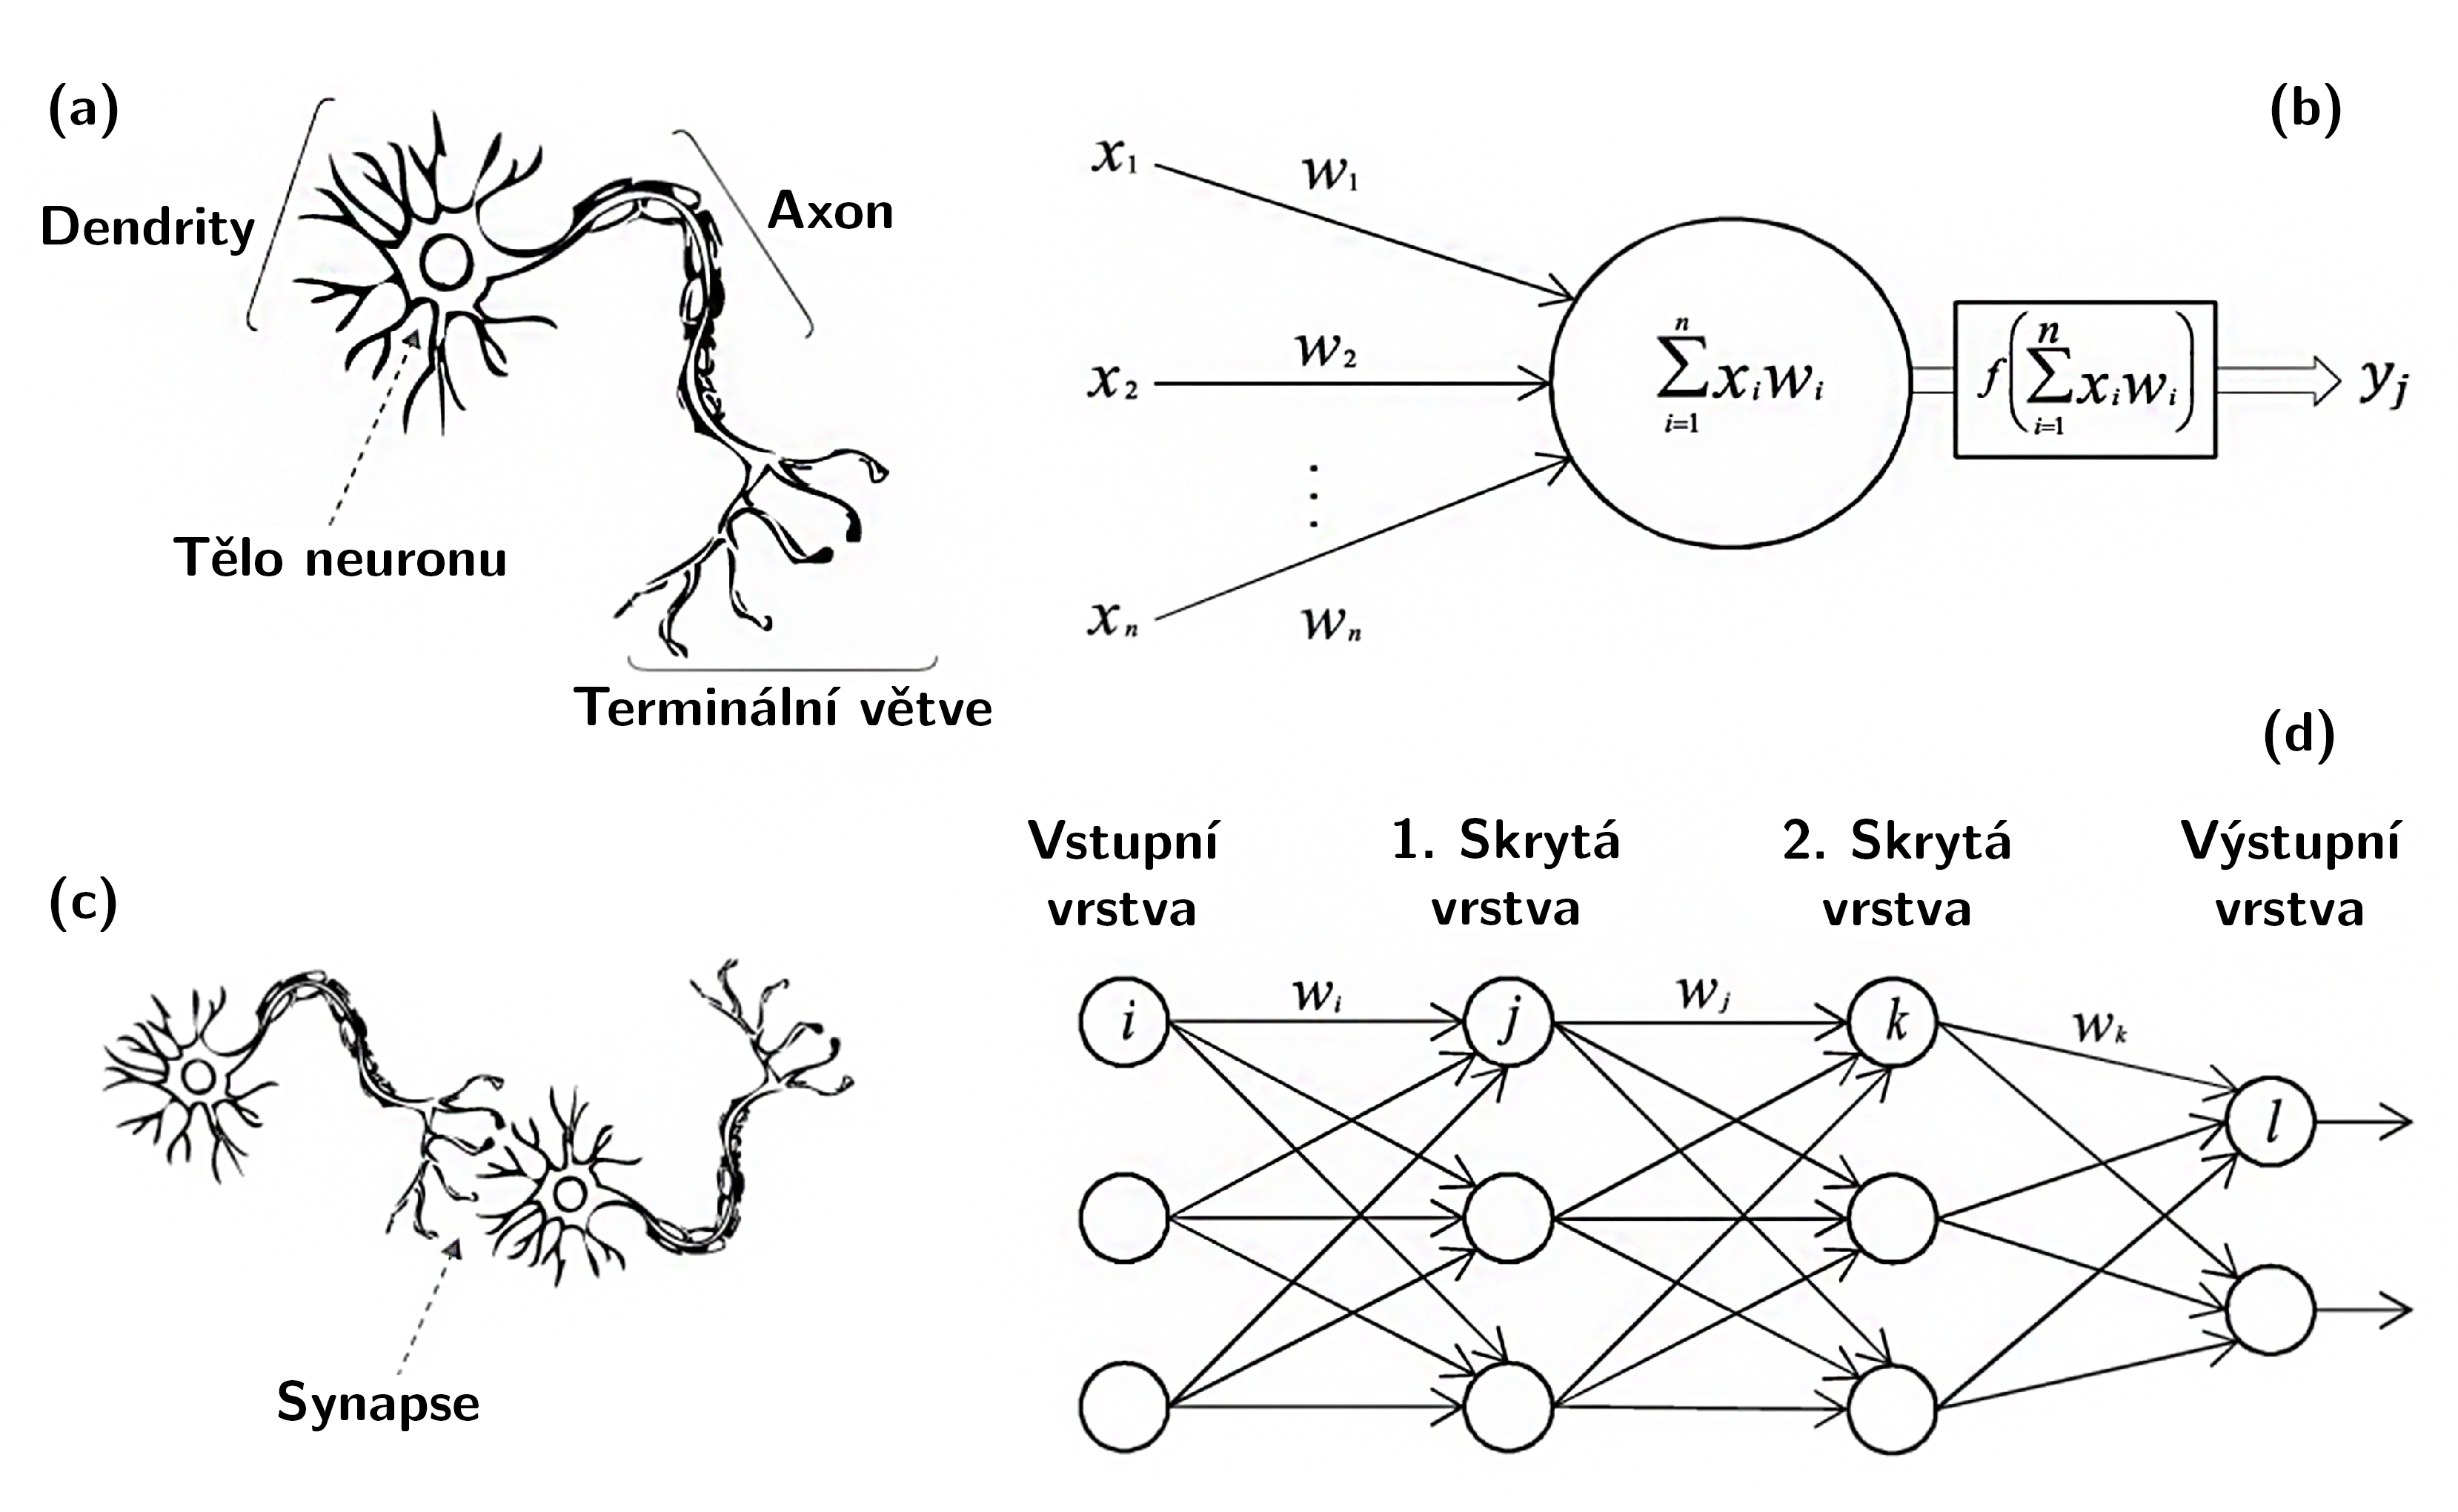
\includegraphics[width=1\linewidth]{figures/ann_comparison_cz}
        \caption{Biologický neuron ve srovnání s umělou neuronovou sítí: \textbf{(a)}
            lidský neuron; \textbf{(b)} umělý neuron; \textbf{(c)} biologická
            synapse; a \textbf{(d)} synapse ANN. (Upraveno a převzato
            z~\cite{suzuki2013})}
        \label{fig:ann_comparison}
    \end{center}
\end{figure}

V průběhu let se \gls{ANN} významně rozvinuly a byly použity k řešení široké
škály úloh. Dnes hrají umělé neuronové sítě klíčovou roli v různých akademických
i komerčních aplikacích při řešení problémů, které jiné metody nezvládají.
Historie a základní koncepty \gls{ANN}, mezi které patří například perceptrony
nebo zpětná propagace a gradientní sestup byly již rozebrány
v~\cite{Aurelien2022,Murphy2012,Goodfellow2016}.

\subsubsection{Ztrátová funkce}
Začátkem této podkapitoly o strojovém učení
(viz~\ref{subsubsec:supervised_learning}) byla definována funkce $h$, před
jejímž hledáním je potřeba učinit předpoklad o jaký typ funkce se jedná
(lineární, polynomická, aj.). Tímto předpokladem vzniká vymezení na určitý
prostor hypotéz, označovaný $\mathcal{H}$, které velmi ovlivňuje generalizaci.

S vymezením přichází na řadu ztrátová funkce $\mathcal{L}:\mathcal{H}
    \rightarrow \mathbb{R}$, jež přiřazuje ztrátu každému $h \in \mathcal{H}$.
    Ztrátu si lze představit jako číslo, které vypovídá o tom jak přesně je
    nalezená $h$ aproximována vzhledem k použitým datům. Se ztrátovou funkcí tak
    vzniká nový optimalizační problem:
\begin{equation}
    \arg\min_{h \in \mathcal{H}} \mathcal{L}(h) = \arg\min_{h \in \mathcal{H}} \frac{1}{n}\sum_{i=1}^nl(\textbf{x}_i,y|h)
\end{equation}
kde $\mathcal{L}$ je ztráta pro danou $h$ v rámci používaných dat a $l$ je
ztráta pro dvojici vstupu a výstupu při dané $h$. Díky takovému způsobu
hodnocení je umožněno modelu se učit. Existuje řada ztrátových funkcí, jejichž
použití závisí na typu problému (regrese, klasifikace, aj.). Tyto funkce
společně s detailnějším popisem optimalizačního problému již byly popsány
v~\cite{Murphy2012}.

\subsubsection{Numerická optimalizace}
Obecně je numerická optimalizace technika, která se používá k nalezení
optimálního řešení výpočetně náročných problémů. Ve strojovém učení se numerická
optimalizace často používá k optimalizaci parametrů modelu. V rámci \gls{ANN} se
k optimalizaci vah spojení mezi neurony běžně využívá gradientní sestup
(\gls{GD}) v různých podobách.

\begin{figure}[h]
    \begin{minipage}{0.55\textwidth}
        \begin{algorithm}[H]
            %\small
            \caption{Gradientní sestup}
            \label{algo:gd}
            \Vst{váhy $w_0$, \# iterací $T$}
            \Vyst{konečné váhy $w_T$}
            \For{$t \in\{0, \ldots T-1\}$}{
                odhad $\nabla \mathcal{L}(w_t)$\\
                výpočet $\Delta w_t = - \nabla \mathcal{L}(w_t)$\\
                výběr rychlosti učení $\gamma$\\
                $w_{t + 1} := w_{t} + \gamma \Delta w_t$
            }
            \Return $w_T$
        \end{algorithm}
    \end{minipage}
    \hspace{10pt}
    \begin{minipage}{0.4\textwidth}
        \centering
        \begin{tikzpicture}[samples=100,smooth]
            \begin{scope}
                \clip(-3.7,-1) rectangle (2.4,4);
                \draw plot[domain=0:360] ({cos(\x)*sqrt(20/(sin(2*\x)+2))},{sin(\x)*sqrt(20/(sin(2*\x)+2))});
                \draw plot[domain=0:360] ({cos(\x)*sqrt(16/(sin(2*\x)+2))},{sin(\x)*sqrt(16/(sin(2*\x)+2))});
                \draw plot[domain=0:360] ({cos(\x)*sqrt(12/(sin(2*\x)+2))},{sin(\x)*sqrt(12/(sin(2*\x)+2))});
                \draw plot[domain=0:360] ({cos(\x)*sqrt(8/(sin(2*\x)+2))},{sin(\x)*sqrt(8/(sin(2*\x)+2))});
                \draw plot[domain=0:360] ({cos(\x)*sqrt(4/(sin(2*\x)+2))},{sin(\x)*sqrt(4/(sin(2*\x)+2))});
                \draw plot[domain=0:360] ({cos(\x)*sqrt(1/(sin(2*\x)+2))},{sin(\x)*sqrt(1/(sin(2*\x)+2))});
                \draw plot[domain=0:360] ({cos(\x)*sqrt(0.0625/(sin(2*\x)+2))},{sin(\x)*sqrt(0.0625/(sin(2*\x)+2))});

                \draw[->,blue,ultra thick] (-2,3.65) to (-1.93,3);
                \draw[->,blue,ultra thick] (-1.93,3) to (-1.75,2.4);
                \draw[->,blue,ultra thick] (-1.75,2.4) to (-1.5,1.8);
                \draw[->,blue,ultra thick] (-1.5,1.8) to (-1.15,1.3);

                \node at (-1.4,3.8){\scriptsize $w[0]$};
                \node at (-1.2,3.2){\scriptsize $w[1]$};
                \node at (-1.05,2.6){\scriptsize $w[2]$};
                \node at (-0.8,2){\scriptsize $w[3]$};
                \node at (-0.6,1.4){\scriptsize $w[4]$};
            \end{scope}
        \end{tikzpicture}
        \caption{Postup \gls{GD}~\cite{gradientdescent}}
        \label{fig:gd}
    \end{minipage}
\end{figure}

Výše lze vidět obecný popis gradientního sestupu (Algoritmus~\ref{algo:gd}).
Jeho cílem je najít minimum funkce tím, že se postupně pohybuje v opačném směru
gradientu funkce. Gradient je vektor, který ukazuje směr největšího nárůstu
funkce. Při pohybu v opačném směru tohoto vektoru, nastává oblast s největší
změnou funkce a lze tedy minimalizovat cílovou funkci. Postupné kroky v opačném
směru gradientu funkce vedou k nalezení optimálního řešení. Na Obr.~\ref{fig:gd}
je vizualizována přirozená aktualizace vah gradientního sestupu ve výstupním
prostoru (pro náhodně inicializovanou síť). Jednotlivé vrstevnice znázorňují
množiny úrovní hodnot ztrátové funkce podél vertikálního a horizontálního směru.
Uprostřed vrstevnic se nachází minimum ztrátové funkce. Z algoritmu výše lze
aktualizaci vah GD popsat následovně:
\begin{equation}
    w_{t+1} = w_t - \gamma \nabla L(w_t)
\end{equation}
kde $w_t$ je aktuální hodnota vektoru vah v čase $t$, $\gamma$ je rychlost učení
(anglicky Learning Rate) a $\nabla L(w_t)$ je gradient cílové funkce v čase $t$.
Různé volby rychlosti učení $\gamma$ a techniky odhadu pro
$\nabla\mathcal{L}(w)$ mohou vést k různým implementacím. Gradientní sestup má
proto řadu variant, včetně stochastického gradientního sestupu a mini-batch
gradientního sestupu, které se liší v způsobu, jakým jsou gradienty vypočítávány
a aktualizovány. Tyto algoritmy již popsal Goodfellow et al.
v~\cite{Goodfellow2016}.

\subsubsection{Aktivační funkce}
Aktivační funkce jsou jednou z nejdůležitějších součástí \gls{ANN}. Tyto funkce
zpracovávají vstupní signály a generují výstupy neuronů, které se dále šíří do
dalších vrstev sítě. Musí také splňovat některé předpoklady jako je
diferencovatelnost. Aktivační funkce musí být také nelineární, aby se rozšířil
rozsah mapovacích funkcí, které lze aproximovat. Existují různé aktivační
funkce, které mají své výhody a nevýhody. Jejich výběr je podstatnou součástí
procesu optimalizace hyperparametrů~\cite{sharma2017,Goodfellow2016}.

\begin{table}[h]
    \centering
    \caption{Vybrané aktivační funkce~\cite{activationfunctions}}
    \label{tab:activationfcn}
    \begin{tabular}{p{1.8cm}p{4.5cm}p{5cm}c}
        \toprule
        \multicolumn{1}{l}{Název} & \multicolumn{1}{l}{Funkce}                               & \multicolumn{1}{l}{Derivace}                                    & \multicolumn{1}{c}{Obrázek} \\
        \midrule
        Sigmoid                   & $\sigma(x)=\frac{1}{1+e^{-x}}$                           & $f'(x)=f(x)(1-f(x))^2$                                          & 
        \multirow{3}{*}{\begin{tikzpicture}[baseline={(0,0.2)}]
                                \draw (-1,0) -- (1,0);
                                \draw (0,0) -- (0,1);
                                \draw plot[domain=-1:1,variable=\x] ({\x},{1/(1+exp(-4*\x))});
                            \end{tikzpicture}}                                                                                                        \\[2ex]
        Softmax                   & $f(x)=\frac{e^x}{\sum_i e^x}$                            & $f'(x)=\frac{e^x}{\sum_i e^x} - \frac{(e^x)^2}{(\sum_i e^x)^2}$ &                             \\
        \\
        tanh                      & $\sigma(x)=\frac{e^x-e^{-x}}{e^z+e^{-z}} $               & $f'(x)=1-f(x)^2$
                                  & \begin{tikzpicture}[baseline={(0,0)}]
                                        \draw (-1,0) -- (1,0);
                                        \draw (0,-1) -- (0,1);
                                        \draw plot[domain=-1:1,variable=\x] ({\x},{tanh(4*\x)});
                                    \end{tikzpicture}                                                                                                  \\
        \\
        ReLU                      & $f(x) =\begin{cases}
                                                   0 & ~\text{if}~ x<0      \\
                                                   x & ~\text{if}~x \geq 0.
                                               \end{cases}$                              & $f'(x)=\begin{cases}
                                                                                                      0 & ~\text{if}~ x<0      \\
                                                                                                      x & ~\text{if}~1 \geq 0.
                                                                                                  \end{cases} $                                     &
        \begin{tikzpicture}[baseline={(0,0.5)}]
            \draw (-1,0) -- (1,0);
            \draw (0,0) -- (0,1);
            \draw plot[domain=-1:1,variable=\x] ({\x},{ifthenelse(\x<0,0,\x)});
        \end{tikzpicture}                                                                                                                   \\ \bottomrule
    \end{tabular}
\end{table}

Logistická funkce, neboli sigmoida, je jednou z nejstarších aktivačních funkcí a
má tvar S-křivky. Sigmoida má nelineární charakter, což umožňuje neuronové síti
modelovat složité vztahy mezi vstupy a výstupy. Nicméně, sigmoida má některé
nevýhody, mezi které patří tzv. \emph{\enquote{vanishing gradient}}, kdy se
gradient funkce blíží nule, což brání učení sítě. Tato funkce také může způsobit
saturaci neuronů, což znamená, že se jejich výstupy blíží k hodnotě 0 nebo 1, a
brání tak dalšímu učení~\cite{sharma2017}.

Hyperbolická funkce tangens (tanh) je podobná sigmoidě, ale má symetrický tvar s
rozsahem mezi -1 a 1. Tanh může být lepší volbou než sigmoida pro určité typy
sítí, protože umožňuje výstupy neuronů, které jsou jak kladné, tak
záporné~\cite{sharma2017}.

Aktivační funkce ReLU (anglicky Rectified Linear Unit) vrací vstupní hodnotu,
pokud je kladná, a nulu, pokud je záporná. Jedná se o velmi populární a
efektivní funkci, která umožňuje rychlé učení sítí. Navíc, ReLU může snížit
výskyt saturace neuronů a dříve zmíněného problému -- \emph{\enquote{vanishing
gradient}}. Nicméně, tato funkce může mít problém s tzv. \emph{\enquote{mrtvými
neurony}}, kdy neuron má výstup vždy roven nule a stává se tak
neaktivní~\cite{sharma2017,Nair2010}.

Leaky ReLU je modifikace ReLU, která řeší problém \emph{\enquote{mrtvých
neuronů}} tím, že má nenulovou hodnotu pro záporné vstupy. Existuje řada dalších
aktivačních funkcí, jako je softmax, která se často používá jako aktivační
funkce pro poslední vrstvu neuronové sítě a používá se v úlohách
klasifikace~\cite{sharma2017}.

\subsubsection{Regularizace}
Z předešlých kapitol vyplývá, že jedním z hlavních cílů učení neuronové sítě je
minimalizace chyby predikce. Často ale dochází k přeučení neuronová sítě, tedy
síť se naučí velmi přesně předpovídat data použitá pro trénování, ale ztrácí
schopnost generalizace. To je způsobeno tím, že síť se snaží přizpůsobit se
každému jednotlivému trénovacímu datovému bodu a následně nedokáže předpovídat
data, která se od těch trénovacích liší. K tomuto jevu dochází, protože
neuronová síť má příliš mnoho parametrů (viz~\ref{subsubsec:underoverfitting}).
Řešením tohoto problému je použití regularizace. Regularizace je technika, která
snižuje rozptyl modelu sítě, a snaží se tak minimalizovat riziko přeučení.
Existuje několik technik regularizace, z nichž nejčastěji používanými jsou L1 a
L2 regularizace, dropout a early stopping.

Metody regularizace L1 a L2 omezují optimalizační metody během procesu
minimalizace ztrátové funkce modelu. Tato omezení penalizují váhy, což vede ke
zjednodušení modelu. Při L1 regularizaci se k nákladové funkci přidává
regularizační člen, který je součtem absolutních hodnot vah. Tento přístup
způsobí, že některé příznaky jsou považovány za méně důležité a je jim přiřazena
nulová váha, čímž se model účinně zjednoduší. Váhy byly dříve indexovány na
základě neuronů a vrstev, které spojují. U L2 je zaveden regularizační člen za
účelem minimalizace součtu čtverců vah. Tento přístup nevede k vynulování vah,
ale snižuje je o faktor úměrný jejich velikosti během každé iterace gradientního
sestupu~\cite{Aurelien2022,Goodfellow2016}.

Dropout je metoda, která náhodně \emph{\enquote{vypne}} některé neurony v síti
během trénování, což má za následek omezení relací mezi neurony a snížení rizika
přeučení. Early stopping je technika, která sleduje vývoj chyby při trénování
sítě na validačním datasetu a zastaví trénování, jakmile se chyba na validačním
datasetu začne zvyšovat. Umožňuje tak včasné ukončení trénování a minimalizaci
rizika přeučení~\cite{Aurelien2022,Goodfellow2016}.